\documentclass[12pt]{ruthesis}

\usepackage{standalone}
\usepackage{graphicx}
\usepackage{hyperref}
\usepackage{listings}
\usepackage{color}
\usepackage{verbatim}
\usepackage{amsmath}
%\usepackage{subfig}
\usepackage{caption}
\usepackage{subcaption}
\usepackage{setspace}
\usepackage{float}
\usepackage{theorem}
\linespread{1.7}

\newtheorem{proposition}{Proposition}

\theoremheaderfont{\itshape} {\theoremstyle{break}
\newtheorem{Fact}{Fact}[chapter]} \theoremstyle{break}
\newtheorem{Lem}{Lemma}[chapter] \theoremstyle{break}
\newtheorem{Thm}{Theorem}[chapter] {\theoremstyle{plain}
  \theorembodyfont{\rmfamily}  \newtheorem{Prf}{Proof}[chapter]}
{\theoremstyle{plain}
  \theorembodyfont{\rmfamily}  \newtheorem{Def}{Definition}[chapter]}

\title{A Multigrid Solver for Graph Laplacian Linear Systems on Power Law Graphs}
\ctitle{A Multigrid Solver for Graph Laplacian Linear Systems on Power Law Graphs}
\author{Eric Buras}
\department{Computational and Applied Mathematics}
\school{Rice University}
\degree{Master of Arts}

\committee {
        Matthew Knepley, Chair \\
        Assistant Professor of Computational and Applied Mathematics \and
        Andrew Schaefer \\
        Noah Harding Chair and Professor of Computational and Applied Mathematics \and
        Anshumali Shrivastava \\
        Assistant Professor of Computer Science       
}

\address{Houston, Texas}
\donemonth{April} \doneyear{2016} \makeindex

\begin{document}
\begin{frontmatter}
   \pagenumbering{arabic}
   %\makecover
   \maketitle
\documentclass{article}

\usepackage{graphicx}
\usepackage{hyperref}
\usepackage{listings}
\usepackage{color}
\usepackage{verbatim}
\usepackage{amsmath}



\begin{document}

\section{Abstract}
The Laplacian matrix, $L$, of a Graph, $G$, contains degree and edge information of a given network. Solving a Laplacian linear system $Lx = b$ provides information about flow through the network, and in specific cases, how that information orders the nodes in the network. I propose a novel way to solve this linear system by first partitioning $G$ into its maximum locally connected subgraph and a small subgraph of the remaining teleportation edges. I then apply optimal MultiGrid solves to the locally connected subgraph, and linear algebra and a solve on the teleportation subgraph to solve the original linear system. I show results for this method on real-world graphs from the biological systems of the \textit{C. Elegans} worm, Facebook friend networks, and the power grid of the Western United States.

%\bibliographystyle{siam}
%\bibliography{mastersbib}


\end{document}
\documentclass{article}

\usepackage{graphicx}
\usepackage{hyperref}
\usepackage{listings}
\usepackage{color}
\usepackage{verbatim}
\usepackage{amsmath}



\begin{document}

\section{Introduction}
In 1999, Stanford graduate students: Larry Page and Sergey Brin proposed a novel algorithm for ordering the information on the world-wide-web. How do you know what links an internet user is likely to follow from any given web-page? Thus, given a network (graph) of connections between web pages, Page and Brin proposed solving a simple linear system resulting in a vector of importances of the web pages for the network. With the shift of a minor parameter, the PageRank linear system was born. Given \textbf{$L$}, a stochastic matrix describing a web graph, \textbf{$b$}, a distribution vector corresponding to the problem data, and $0 < \alpha < 1$, a damping parameter; solve the linear system:\\
\begin{center}
$(I-\alpha L)x = (1-\alpha)b$ \cite{Page:1999} \\
\end{center}
for \textbf{$x$}, the PageRank vector. This solution contains information about the importance of a set of web-pages on the internet. The $\alpha$ parameter is used to introduce likelihood that a user clicks on a new random page \cite{Page:1999}.\\
\\
While Page and Brin went on to make billions of dollars revolutionizing web-search, their algorithm can be thought of in more generic terms for any network of information. David Gleich highlights other applications of the PageRank linear system in his paper reviewing it's simple mathematics and vast reach into other, completely different topics \cite{Gleich:2015}. These include chemical bonding networks, macro and micro biological system networks, roads and infrastructural networks, computer hardware and software networks, author and literature networks, and finally social organization networks \cite{Gleich:2015}. Scientists care deeply about the information inherent in the connections of these networks, and finding a way to order that information in a suitable format. Thus PageRank linear systems become GeneRank \cite{Jiang:2009}, AuthorRank \cite{Liu:2005}, or MonitorRank \cite{Kim:2013} linear systems for information stored in genes, co-authorships, and distributed system logs, respectively \cite{Gleich:2015}. The simplicity of the problem formulation combined with the vast amounts of data in practically any subject area shows how influential PageRank has become.\\
\\
The purpose of this paper is to propose a new method for solving a simple linear system similar to that of PageRank. By utilizing the structure of a graph of a certain class, I split the graph into a large, highly locally-connected subgraph and a much smaller subgraph of the remaining teleportation edges. I solve the overall linear system by optimally solving the local subgraph using the Algebraic Multigrid method, and combining linear algebra and a much smaller system solve for the teleportation subgraph. This is a new way of solving a complete graph linear system by breaking it down into smaller problems yet still retaining all available information from the graph.

%\bibliographystyle{siam}
%\bibliography{mastersbib}
\end{document}
\documentclass{article}

\usepackage{graphicx}
\usepackage{hyperref}
\usepackage{listings}
\usepackage{color}
\usepackage{verbatim}
\usepackage{amsmath}



\begin{document}

\section{Background}
\subsection{Graph Laplacian Problem}
Information about a weighted, undirected graph $G$ with vertex list $V$ and edge list $E$ can be stored in a matrix. This is called the adjacency matrix which is defined as:\\
\begin{center} 
$A(u,v) = 1$ if $(u,v) \in E$ and $0$ otherwise.\\
\end{center}
The diagonal matrix, $D$ is a matrix of the degree sequence along the diagonal:\\
\begin{center}
$D(u,u) = d_u$
\end{center}
The laplacian matrix is $L = D-A$. This is done because it is similar to the finite difference discretization of the laplacian on a grid (cite?). To see how information flows through paths in a network, the graph laplacian matrix can be used as an operator on an input vector. To find a weighted average of paths in a network one can repeatedly apply the laplacian operator on an input:\\
\begin{center}
$b + Lb + L^{2}b + L^{3}b + L^{4}b + ... = \sum_{i = 0}^{\infty} L^{i}b = (I-L)^{-1}b$\\
\end{center}
Thus in problems related to graph regression, spectral graph theory, maximum and minimum cost flow, resistor networks, and partial differential equations it is common to use the inverse operator of the graph laplacian. \cite{Spielman:2010}

\subsection{Current Solution Approaches}
Solution algorithms for linear systems can be divided into direct methods and iterative methods. Standard direct methods such as $LU$ or Cholesky factorization are accurate and suitable for graphs with small numbers of edges/vertices, however become very costly in terms of memory and time as the size and edge density of the graph increases. Fast matrix inversion can be applied with order $O(n^{2.376})$ \cite{Spielman:2010}, yet this can be improved upon still. Alternatively one can use nested dissection, however computational memory requirements blow up as size increases \cite{Khaira:1992}. In contrast to direct solvers, iterative methods compute better and better approximate solutions to the linear system. A standard iterative method is the Conjugate Gradient method \cite{Hestenes:1952}. To speed up these iterative methods, it is possible to introduce a preconditioner that creates an equivalent linear system that is much easier to solve than the original \cite{Saad:2003}. Yet none of these basic solvers take into account attributes of the graph Laplacian that can drastically improve method performance.

\subsubsection{Spielman-Teng, Koutis et. al.}
An analogy with preconditioning, we want to find an approximation to a graph $G$ with similar spectrum for easier computing. Spielman and Teng introduce the idea of a spectral sparsifier. The Laplacian for this approximation is similar to the Laplacian for the original graph because of similar spectrum, thus resulting in a good preconditioner for the original linear system. Multiple cycles of sparsification and factorization combine to solve the original problem. They have a multilevel version of this. Spielman and Teng (S-T) were thus able to solve symmetric diagonally dominant systems in nearly linear time \cite{Spielman:2008}.  This line of work combined with Vaidya's \cite{Vaidya:1991} work on subgraph preconditioners (capacitance matrix methods) resulted in Koutis and Miller's work solving linear systems based on planar Laplacians \cite{Koutis:2007}. Koutis, et. al. were then able to further decrease the time complexity of S-T for general symmetric diagonally dominant systems \cite{Koutis:2010}.

\subsubsection{Multigrid Approaches}
Algebraic Multigrid utilizes a Galerkin operator in multiple graph coarsening cycles to solve a linear system. It is mostly used to solve discretized partial differential equations, but has also become more popular in solving graph Laplacian systems. AMG has optimal time complexity and demonstrates good parallel scaling thus it is useful for solving incredibly large problems \cite{Livne:2012}. Three current multigrid approaches are combinatorial multigrid (CMG) from Koutis et. al., Cascadic multigrid from Urschel et. al., and Lean Algebraic Multigrid (LAMG) from Livne and Brandt. All three propose coarsening over the entire graph, but an important question to ask is: how do you coarsen a graph with edges of varying degrees? How do you know which edges or vertices can be aggregated and still preserve information?


\subsubsection{Combinatorial Multigrid (CMG)}
Koutis, Miller, and Tolliver propose a combinatorial multigrid solver to solve computer vision problems. This method creates a two-level iterative approach combining the previously mentioned subgraph preconditioning work of Vaidya with algebraic multigrid. For a set of increasingly larger three-dimensional images, CMG required less iterations to converge than a standard multigrid solver in Matlab \cite{Koutis:2011}.

\subsubsection{Lean Algebraic Multigrid (LAMG)}
Livne and Brandt ran a "lean" multigrid algorithm on graph Laplacian systems for almost 4000 real world graphs of varying size and in vastly different fields from the natural sciences to social networks. Their method has three key parts: first, vertices with low degree are eliminated before the graph is coarsened. Second: they aggregate vertices for the coarsening by a proximity heuristic. And third: they apply an energy correction to the Galerkin operator and combine iterate solutions for more accuracy. They test their algorithm against CMG, and find that it requires slightly more work, however is more robust overall \cite{Livne:2012}.One potential downside of LAMG is the vertex aggregation step of multigrid. How can vertices be evenly aggregated over graphs with uneven degree distribution?


\subsubsection{Cascadic Multigrid}
A final alternative form of multigrid was proposed by Urshel et. al. to solve a related problem to the graph Laplacian linear system; they wanted to calculate the Fiedler vector (eigenvector corresponding to the second smallest eigenvalue) of a graph Laplacian. This cascadic multigrid utilizes heavy edge maching to quickly coarsen a graph \cite{Urschel:2014}. It remains to be seen whether this approach will be successful for solving an entire Laplacian linear system accurately.

\subsection{Graph Partitioning and Multigrid}
I have studied the methods of graph partitioning and sparsification for solving linear systems, and using multigrid to solve the graph laplacian linear system specifically. I combine these two approaches using Chung and Lu's work \cite{Chung:2004} and optimal multigrid to solve similar linear systems.
%\bibliographystyle{siam}
%\bibliography{mastersbib}


\end{document}
\documentclass{article}

\usepackage{graphicx}
\usepackage{hyperref}
\usepackage{listings}
\usepackage{color}
\usepackage{verbatim}
\usepackage{amsmath}



\begin{document}
\title{Eric Buras Thesis: Methodology}

\maketitle

\section{Graph Partitioning}
In studying 'small world' networks proposed by Watts and Strogatz \cite{Watts:1998} Fan Chung and Linyuan Lu propose an algorithm that separates a graph into a locally connected component and a global component. Finding a local subgraph is akin to finding a locally connected portion of a graph. Given integers $k \geq 2$ and $l \geq 2$, a $(k,l)$ locally connected graph will have at least $l$ paths connecting any given two nodes with distinct edges in each path. The length of each path can be at most $k$ edges for this pair. A grid network can be described locally with $k=3, l=3,$ and $k=5, l=9$ and is a good example of how connected these types of graphs are. Given graph $G$, its maximum locally connected subgraph is the union of all locally connected subgraphs within the entire graph. It is important that this maximum is unique, and can be found through edge deletion \cite{Chung:2004}. Thus we are able to split a graph into two unique components.\\

(Picture of grid graph with random edges and graph split)\\

\section{Laplacian Solver}
I have partitioned a graph into its locally connected subgraph, $P$ , and the graph of the teleportation edges, $T$. These subgraphs can be converted to Laplacian form with $P_L$ matrix of connections and degree information for the locally connected part, and $T_L$, similar for the teleportation part. With a minor diagonal operation on $T_L$, we have $L = P_L + T_L$ where $L$ is the Laplacian for the entire graph. To solve a Laplacian linear system $Lx=b$ we now solve the two subgraph Laplacians and use linear algebra.

\section{Algebraic Multigrid of Locally Connected Subgraph}
The locally connected subgraph is planar, meaning it can be drawn on a piece of paper without any edges crossing (proof it is planar?). Using work beginning with Gary Miller \cite{Miller:1995}, we know that an Algebraic Multigrid solver is optimal for this planar graph laplacian matrix as the solution space is split into multiple cycles of coarsened solving \cite{Brandt:1984}. This solves $P_L y=b$ where b is the right hand side of the original linear system. Previous approaches to using multigrid to solve Laplacian linear systems do not have a systematic method of graph coarsening. Thus they are prone to losing edge information in the multiple coarsening cycles. (do i need to cite?)

\section{Low Rank SVD of Teleportation Subgraph}
For graphs I am interested in, the number of edges in the Teleportation subgraph is very small relative to the size of the original graph. This causes the laplacian matrix, $T_L$, to have very low rank structure. I can then take the low rank singular value decomposition (cite?) to solve this small portion. This part of the algorithm takes negligible time relative to the multigrid cycles on the planar portion.

\section{Linear Algebra: Woodbury Matrix Identity}
To combine the SVD and Multigrid solves, I utilize the Woodbury matrix Identity:\\
\begin{center}
$(A+UCV)^{-1} = A^{-1} - A^{-1}U(C^{-1}+VA^{-1}U)^{-1}VA^{-1}$\\
\end{center}
with A replaced by $P_L$, $U$ and $V$ component matrices of the SVD of $T_L$, and $C$ replaced by a diagonal of the singular values of $T_L$.

\section{Summary of Solving the Laplacian Linear System}
\begin{center}
$Lx=b$\\
$x = L^{-1}b$\\
$x = (P_L+T_L)^{-1}b$\\
$x = (P_L+USV)^{-1}b$\\
Use Woodbury matrix identity\\
$x = (P_L^{-1}-P_L^{-1}U(S^{-1}+VP_L^{-1}U)^{-1}VP_L^{-1})b$\\
$x = P_L^{-1}b-P_L^{-1}U(S^{-1}+VP_L^{-1}U)^{-1}VP_L^{-1}b$\\
\end{center}

\section{Complexity of Graph partitioning and Linear System Solve}
NEED THIS

\section{NetworkX and PETSc}
NetworkX is a valuable library for graph theory and analysis written in python. This library has many functions for working with data, and specifically use the kl\_ connected\_subgraph function to partition the graph into the locally connected subgraph and the teleportation subgraph. \cite{Hagberg:2008} This function operates according to Chung and Lu's greedy algorithm. Currently this function operates in serially over the graph edges,  and I believe there is ample opportunity to speed it up.\\
The Portable, Extensible Toolkit for Scientific Computation (PETSc) is primarily written in C for solving partial differential equations, however there is a library for python users called petsc4py \cite{Dalcin:2011}. I utilize the algebraic multigrid solvers in PETSc for the locally connected subgraph solves as mentioned above \cite{petsc-user-ref}.






\bibliographystyle{plain}
\bibliography{mastersbib}
\end{document}
\documentclass{article}

\usepackage{graphicx}
\usepackage{hyperref}
\usepackage{listings}
\usepackage{color}
\usepackage{verbatim}
%\usepackage{subfigure}
\usepackage{amsmath}
\usepackage{caption}
\usepackage{subcaption}



\begin{document}
\title{Eric Buras Thesis: Results}

\maketitle

\section{Graphs}
We have a set of graphs that are similar to the power-law graphs from Watts-Strogatz and Chung-Lu. These encompass a wide range of subjects such as social networks, biological processes, and an electric grid. The key part of my algorithm is partitioning a graph into a large locally-connected subgraph and a small teleportation subgraph. four of these examples fully fit into this class of graphs, whereas the power grid most certainly does not as evidenced below. The important attribute to look for is low rank of the teleportation Laplacian matrix relative to the number of the nodes (which is the size of the entire square Laplacian matrix).\\


\begin{figure}
\centering

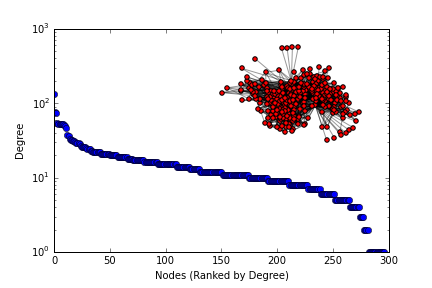
\includegraphics[width=\linewidth]{neural_degree_histogram.png}
\caption{Neural Network of C. Elegans \cite{White:1986,Watts:1998}}
  
\end{figure}

\begin{figure}
\centering
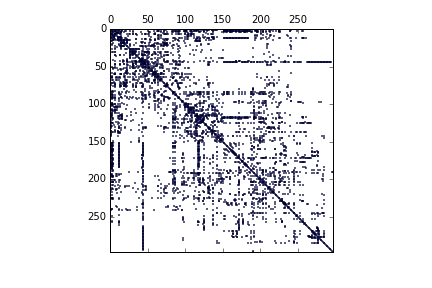
\includegraphics[width = \linewidth]{neuralspy.png}
\caption{Spy Plot of Neural Network Laplacian Matrix}
\end{figure}

\begin{figure}
\centering

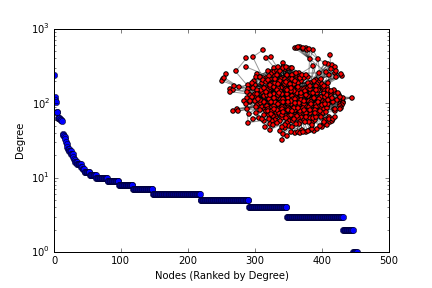
\includegraphics[width=\linewidth]{meta_degree_histogram.png}
\caption{Metabolic Network of C. Elegans \cite{Duch:2005}}
  
\end{figure}
\begin{figure}
\centering
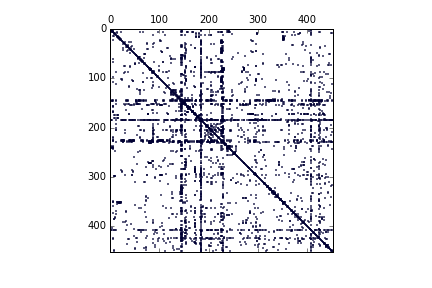
\includegraphics[width = \linewidth]{metaspy.png}
\caption{Spy Plot of Metabolic Network Laplacian Matrix}
\end{figure}

\begin{figure}
\centering

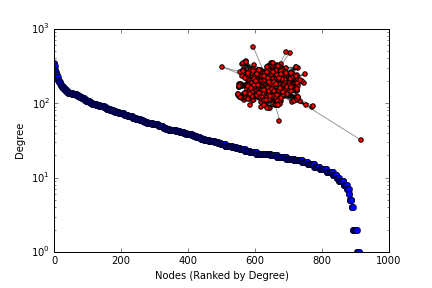
\includegraphics[width=\linewidth]{gene_degree_histogram.png}
\caption{Gene Network Encoding Proteins of C. Elegans \cite{Simonis:2009}}
  
\end{figure}

\begin{figure}
\centering
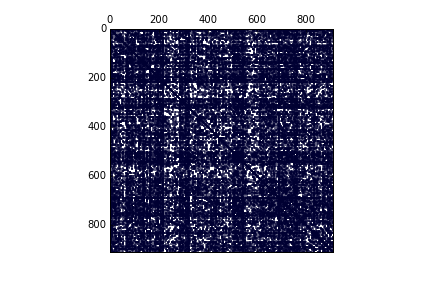
\includegraphics[width = \linewidth]{genespy.png}
\caption{Spy Plot of Gene Network Laplacian Matrix}
\end{figure}

\begin{figure}
\centering

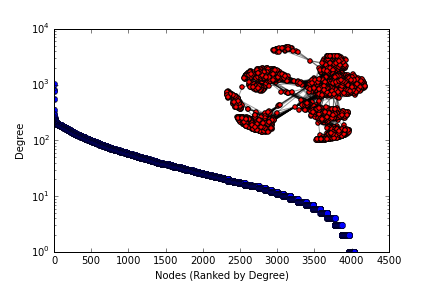
\includegraphics[width=\linewidth]{fb_degree_histogram.png}
\caption{Facebook Friend Network \cite{Mcauley:2012}}
  
\end{figure}

\begin{figure}
\centering
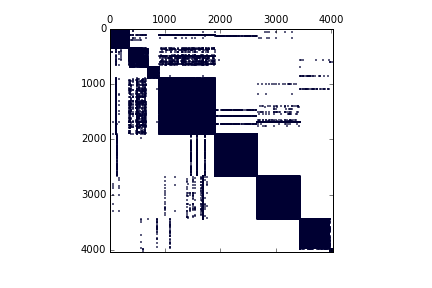
\includegraphics[width = \linewidth]{fbspy.png}
\caption{Spy Plot of Facebook Network Laplacian Matrix}
\end{figure}

\begin{figure}
\centering

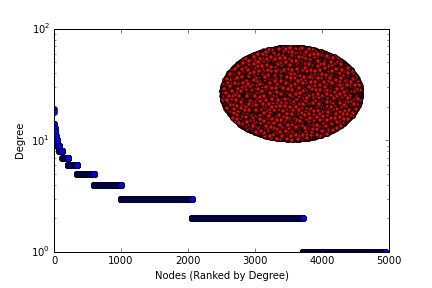
\includegraphics[width=\linewidth]{power_degree_histogram.png}
\caption{Network of Western Power Grid \cite{Watts:1998}}
  
\end{figure}

\begin{figure}
\centering
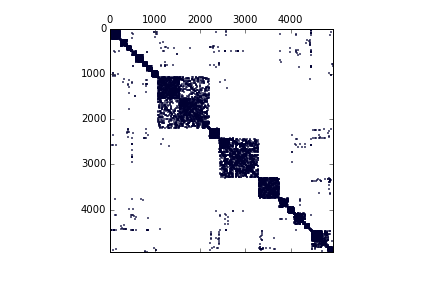
\includegraphics[width = \linewidth]{powerspy.png}
\caption{Spy Plot of Power Grid Laplacian Matrix}
\end{figure}


\begin{center}
\renewcommand{\arraystretch}{1.5}
    \begin{tabular}{| l | l | l | l | l | l |}
    \hline
    Graph (nodes, edges) & Avg. Deg. & Rank $T_L$ & Nx part. (s) & Part. (s) & Iter. \\ \hline
    Neural (297, 2148) & 14.46 & 22 & 11 & 1.6 & 2 \\ \hline
    Metabolic (453, 2025) & 8.94 & 49 & 12 & 2.3 & 2 \\  \hline
    Gene (912, 22738) & 49.86 & 26 & 1915 & 53 & 1 \\ \hline
    Facebook (4039, 88234) & 43.69 &  180 & 11593 & 480 & 2 \\ \hline
    Power (4941, 6594) & 2.669 & 4284 & 2.1 & .33 & 2 \\ 
    \hline
    \end{tabular}
\end{center}
I want to dig deeper into the solve portion to determine if the operations correspond with their given theoretical complexities. Here is a table of the timings for the individual operations:\\

\begin{center}
\renewcommand{\arraystretch}{1.5}
    \begin{tabular}{ | l | l | l | l | l | l | l |}
    \hline
    \textbf{Operation} & \textbf{Order} & \textbf{Neural} & \textbf{Meta} & \textbf{Gene} & \textbf{FB} & \textbf{Power} \\ \hline
    $USV = T_L$ & $O(n^3)$ & .0334 & .0737 & .4183 & 38.47 & 72.86  \\ \hline
    $S^{-1}$ & $O(r)$ & .0005 & .0007 & .0001 & .0023 & 5.104 \\ \hline
    $y = P_L^{-1}b$ (MG) & $O(n)$ & .0857 & .0962 & .3552 & 1.347 & .1152  \\  \hline
    $y_1 = Vy$ & $O(rn)$ & .0013 & .0015 & .0002 & .0023 & .0702 \\ \hline
    $Q = P_L^{-1}U$ ($r\times$MG) & $O(rn)$ & .3292 & .7360 & .5190 & 23.11 & 106.9  \\ \hline
    $Q_1 = VQ$ & $O(r^2 n)$ & .0006 & .0036 & .0013 & .4124 & 285.1 \\ \hline
    $Q_2 = S^{-1} + Q_1$ & $O(r^2)$ & .0012 & .0018 & .0003 & .0011 & .4157 \\ \hline
    $y_2 = Q_2^{-1}y_1$ & $O(r^3)$ & .0023 & .0025 & .0013 & .0099 & 86.49 \\ \hline
    $y_3 = Uy_2$ & $O(rn)$ & .0001 & .0002 & .0003 & .0025 & .1867 \\ \hline
    $y_4 = P_L^{-1}y_3$ (MG) & $O(n)$ &.0128 & .0070 & .1183 & .8249 & .0059 \\ \hline
    $x = y - y_4$ & $O(n)$ &.0003 & .0003 & .0003 & .0004 & .0003 \\ \hline
    \textbf{Total} & $O(n^3)$ & .51 & .966 & 1.44 & 64.46 & 560 \\
    \hline
    \end{tabular}
\end{center}
As observed, the operation timings correspond to their theoretical floating point operation orders. For the first four examples (not including the power grid solve), the limiting operations are the singular value decomposition and multiple right hand side multigrid solves, $Q = P_L^{-1}U$. These operations can be optimized using the low-rank SVD and by vectorizing the multiple right hand solves so that only one multigrid solve must be done. However for the full rank power-grid solve, the limiting operations are the SVD, the matrix-matrix multiplication, $Q_1 = VQ$, and the matrix solve, $y_2 = Q_2^{-1}y_1$. Graph Laplacian linear systems without low-rank $T_L$ should not be solved using this method.

\bibliographystyle{plain}
\bibliography{mastersbib}
\end{document}
\documentclass{article}

\usepackage{graphicx}
\usepackage{hyperref}
\usepackage{listings}
\usepackage{color}
\usepackage{verbatim}
%\usepackage{subfigure}
\usepackage{amsmath}
\usepackage{caption}
\usepackage{subcaption}
\usepackage{placeins}
\usepackage{setspace}
\usepackage{float}

\linespread{1.5}

\begin{document}

\section{Dataset Figures}
\subsection{\textit{C. Elegans} Neural Network}
\begin{figure}[H]
\centering

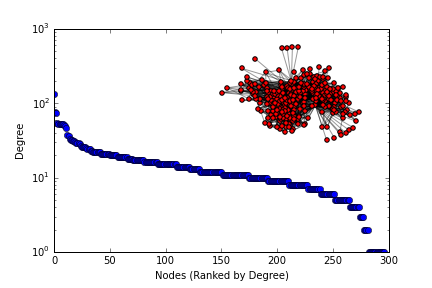
\includegraphics[width=.8\linewidth]{neural_degree_histogram.png}
\caption{Neural Network of \textit{C. Elegans}}
  
\end{figure}

\begin{figure}[H]
\centering
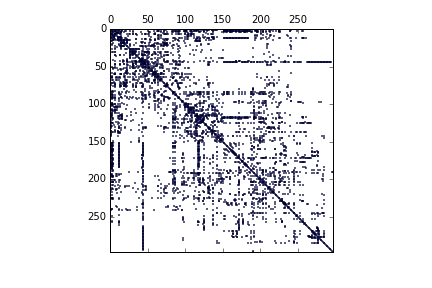
\includegraphics[width = \linewidth]{neuralspy.png}
\caption{Spy Plot of Neural Network Laplacian Matrix}
\end{figure}
\begin{figure}[H]
\centering
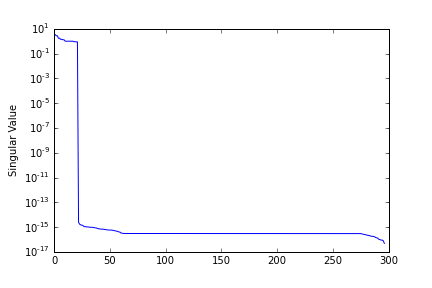
\includegraphics[width = .9\linewidth]{neuralsing.png}
\end{figure}


\subsection{\textit{C. Elegans} Metabolic Network}
\begin{figure}[H]
\centering

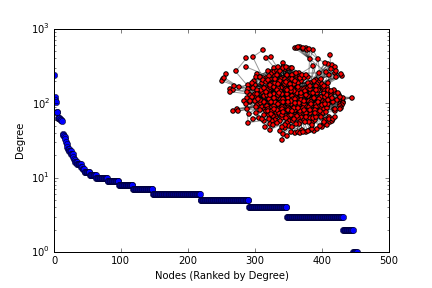
\includegraphics[width=.8\linewidth]{meta_degree_histogram.png}
\caption{Metabolic Network of \textit{C. Elegans}}
  
\end{figure}
\begin{figure}[H]
\centering
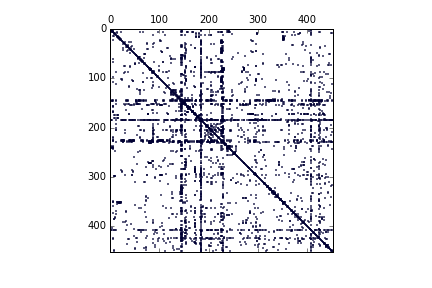
\includegraphics[width = \linewidth]{metaspy.png}
\caption{Spy Plot of Metabolic Network Laplacian Matrix}
\end{figure}
\begin{figure}[H]
\centering
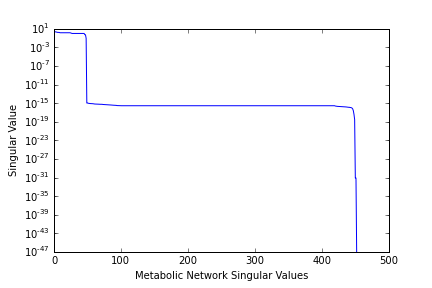
\includegraphics[width = .9\linewidth]{metasing.png}
\end{figure}


\subsection{\textit{C. Elegans} Protein Network}
\begin{figure}[H]
\centering

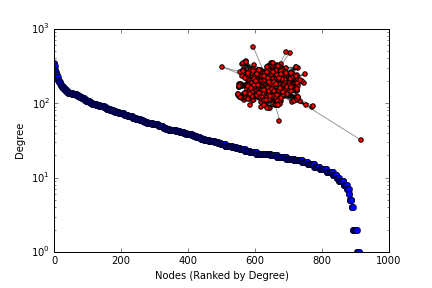
\includegraphics[width=.8\linewidth]{gene_degree_histogram.png}
\caption{Protein Network with Corresponding Phenotypes of \textit{C. Elegans}}
  
\end{figure}

\begin{figure}[H]
\centering
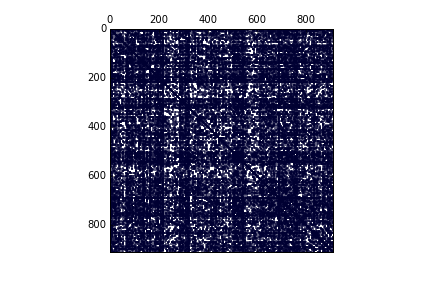
\includegraphics[width = \linewidth]{genespy.png}
\caption{Spy Plot of Protein Network Laplacian Matrix}
\end{figure}
\begin{figure}[H]
\centering
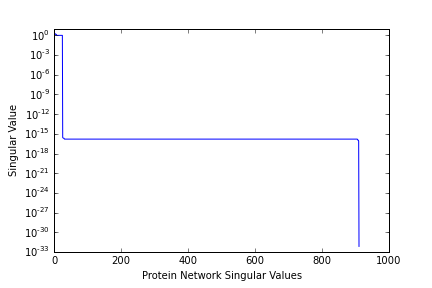
\includegraphics[width = .9\linewidth]{proteinsing.png}
\end{figure}


\subsection{Facebook Friend Network}
\begin{figure}[H]
\centering

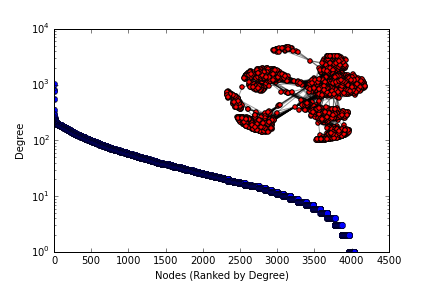
\includegraphics[width=.8\linewidth]{fb_degree_histogram.png}
\caption{Facebook Friend Network}
  
\end{figure}

\begin{figure}[H]
\centering
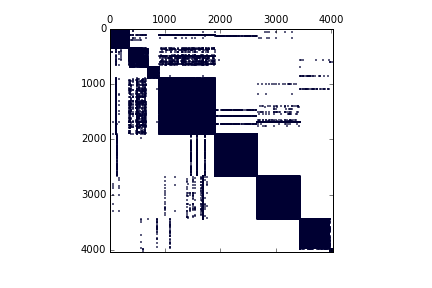
\includegraphics[width = \linewidth]{fbspy.png}
\caption{Spy Plot of Facebook Network Laplacian Matrix}
\end{figure}
\begin{figure}[H]
\centering
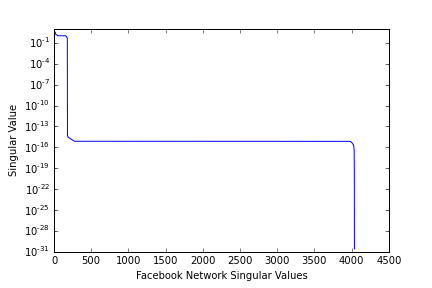
\includegraphics[width = .9\linewidth]{fbsing.png}
\end{figure}


\subsection{Power Grid}

\begin{figure}[H]
\centering

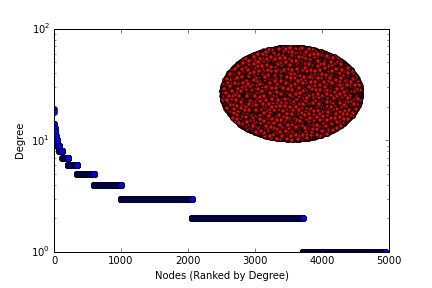
\includegraphics[width=.8\linewidth]{power_degree_histogram.png}
\caption{Network of Western Power Grid}
  
\end{figure}

\begin{figure}[H]
\centering
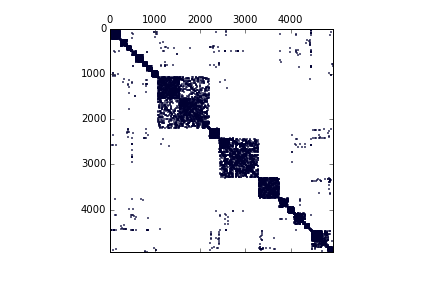
\includegraphics[width = \linewidth]{powerspy.png}
\caption{Spy Plot of Power Grid Laplacian Matrix}
\end{figure}

\begin{figure}[H]
\centering
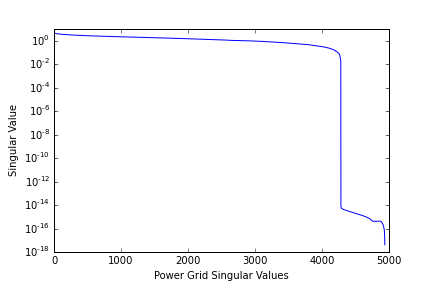
\includegraphics[width = .9\linewidth]{powersing.png}
\end{figure}

\end{document}

\documentclass{article}

\usepackage{graphicx}
\usepackage{hyperref}
\usepackage{listings}
\usepackage{color}
\usepackage{verbatim}
\usepackage{amsmath}

\linespread{1.5}


\begin{document}

\section{Conclusions and Future Work}
In conclusion I have utilized maximum locally-connected subgraph partitioning from Chung-Lu to partition a graph into a planar subgraph and a teleportation subgraph. I then combine optimal multigrid solves on the planar subgraph with linear algebra and a direct solve on the teleportation subgraph. I have now solved the original laplacian linear system in a simple and straightforward manner that can be replicated easily. I give a complexity model for the partitioning algorithm, $O(num\_iter. \times num\_edges \times E[d]^3)$, and a suboptimal complexity for the linear system solve, $O(num\_nodes^3)$. Using the Woodbury matrix identity \cite{Woodbury:1950} I solve the laplacian linear systems for biological networks of \textit{C. Elegans}, for Facebook friend circles, and show how my method does not work for the power grid of the Western US. The individual operations align with their theoretical computational cost. However, there is much to continue working on.

\subsection{Graph Partitioning}
My graph partitioning algorithm is written in python mainly because of ease-of-use and because of the NetworkX library that provides simple graph computations. However I can rewrite much of the code in C to efficiently create graph structs. I can then test local-connectivity for edges in parallel, drastically decreasing time to partition. I would also like to submit my graph partitioning algorithm to the open source NetworkX library as an alternative to the k,l\_connected\_subgraph function for small $k$ \cite{Hagberg:2008}.
\subsubsection{Theoretical Bounds}
In addition to working on the code for the algorithm, I would like to work with graph theorists to really classify graphs with large locally-connected components. There might be bounds on the size of the teleportation subgraph which can lead to bounds on the rank of the teleportation laplacian matrix. This could help establish a class of graphs for which my method is appropriate.

\subsection{Linear System Solve}
Most of my code is built on PETSc which is written in C and optimized for sparse matrices \cite{petsc-user-ref} however the initial singular value decomposition is computed using numpy and does not utilize the low-rank ($r$) nature of the teleportation laplacian matrix. This results in $O(n^3)$ operations instead of $O(r^{2}n)$ operations. Also, PETSc does not have a vectorized multiple right-hand-side solve technique that will drastically decrease computations for the $Q_1 = VQ$ step in the linear system solve that is causing a bottleneck. If I implement this, I can speed up the system solve.

\subsection{Larger Graphs and Finding Meaningful Solutions}
I only tested my method on graphs of small to medium size due to memory constraints on my laptop. I would like to test these and much larger graphs on a cluster to determine how my method scales. Because I am especially interested in biological systems, I would like to test my method on more complex systems than \textit{C. Elegans}.\\
 \\
Finally, and most importantly, I did not have enough time to truly evaluate solutions to the laplacian linear systems for my example graphs. I need to do more work to find appropriate right hand sides to solve against. Currently I am solving against a random right hand side. What are the most important regions of the worm's nervous system? Are there any hidden protein-phenotype expressions that could be important in unraveling the worm's genome? Who are the origins of influence in the Facebook friend networks? These are the real questions scientists are asking, I have proposed a method to answer them, and would like to see the final results.
%\bibliographystyle{siam}
%\bibliography{mastersbib}
\end{document}

\end{frontmatter}
\begin{spacing}{1}
\pagenumbering{roman}
\bibliographystyle{siam}
\bibliography{mastersbib}
\end{spacing}
\end{document}